\documentclass[12pt,a4paper]{article}
\usepackage[UTF8]{ctex}
\usepackage{amsmath,amssymb}
\usepackage{xcolor}
\usepackage{hyperref}
\usepackage{geometry}
\usepackage{graphicx}
\geometry{margin=2.5cm}

\title{Dynamic QAOA / 动态量子近似优化算法}
\author{QuoNic}
\date{}

\begin{document}
\maketitle

\begin{center}
\textbf{Algorithms / 算法} | 难度：高级 | 预计时间：20 分钟
\end{center}

\tableofcontents
\newpage

\section{为什么需要？}

动态 QAOA 是 QAOA 的改进版本，使用动态参数调整来提高优化效果。

\subsection{经典局限}
\begin{itemize}
  \item 标准 QAOA 的参数优化困难
  \item 对于复杂问题，标准 QAOA 收敛慢
\end{itemize}

\subsection{量子优势}
\begin{itemize}
  \item 动态 QAOA 可以自适应调整参数
  \item 收敛速度更快
  \item 可以处理更复杂的问题
\end{itemize}

\subsection{实际应用}
\begin{itemize}
  \item 组合优化
  \item 机器学习
  \item 量子化学
\end{itemize}

\section{快速上手}

\begin{verbatim}
from quonic.algorithms import dqaoa

# 动态 QAOA
graph = [(0,1), (1,2), (2,0)]
result = dqaoa(graph, p=2, adaptive=True)
print(f'MaxCut: {result.maxcut_value}')
\end{verbatim}

\textbf{预期输出}：
\begin{verbatim}
MaxCut: 2
\end{verbatim}

\section{原理详解}

\subsection{电路图}

\begin{center}
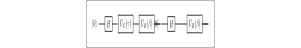
\includegraphics[width=0.6\textwidth]{../../images/dqaoa_circuit.svg}
\end{center}

\subsection{数学推导}

动态 QAOA：
\begin{equation}
|\gamma(t), \beta(t)\rangle = \prod_{l=1}^{p} e^{-i\beta_l(t) B} e^{-i\gamma_l(t) C} |+\rangle^{\otimes n}
\end{equation}

\textbf{动态参数}：
\begin{equation}
\gamma_l(t+1) = \gamma_l(t) + \eta \nabla_\gamma F
\end{equation}

\subsection{几何解释}

动态 QAOA 在参数空间中自适应调整参数。量子叠加允许同时探索多个参数路径。

\section{代码详解}

\begin{verbatim}
from quonic.algorithms import dqaoa

# dqaoa(graph, p, adaptive)
# graph: 图的边列表
# p: QAOA 层数
# adaptive: 是否使用动态参数
result = dqaoa(graph, p=2, adaptive=True)

# result.maxcut_value: MaxCut 值
# result.solution: 最优解
# result.params: 动态参数
print(f'MaxCut: {result.maxcut_value}')
\end{verbatim}

\section{进阶用法}

\subsection{场景 1：不同层数}

\begin{verbatim}
from quonic.algorithms import dqaoa

for p in [1, 2, 4]:
    result = dqaoa(graph, p=p, adaptive=True)
    print(f'p={p}: MaxCut={result.maxcut_value}')
\end{verbatim}

\section{适用场景}

\subsection{组合优化}

动态 QAOA 可以用于求解 MaxCut、旅行商问题等组合优化问题。动态参数调整可以提高优化效果，加速收敛。

\subsection{机器学习}

动态 QAOA 可以用于量子机器学习中的特征选择、参数优化等。动态参数调整可以提高学习效率。

\section{常见问题}

\subsection{动态 QAOA 和标准 QAOA 有什么区别？}

动态 QAOA 使用动态参数调整，可以自适应地优化参数，收敛速度更快。

\subsection{动态 QAOA 的精度如何？}

精度取决于层数和参数调整策略。

\section{学习路径}

\subsection{前置知识}
\begin{itemize}
  \item QAOA
  \item 组合优化
  \item 参数优化
\end{itemize}

\subsection{继续学习}
\begin{itemize}
  \item 量子优化
  \item 量子机器学习
  \item 量子化学
\end{itemize}

\section{完整示例代码}

\subsection{示例 1：基本动态 QAOA}

\begin{verbatim}
from quonic.algorithms import dqaoa

graph = [(0,1), (1,2), (2,0)]
result = dqaoa(graph, p=2, adaptive=True)
print(f'MaxCut: {result.maxcut_value}')
\end{verbatim}

\section{下载}

\begin{itemize}
  \item [dqaoa.py](https://github.com/ChrisLee0721/QuoNic/blob/main/examples/dqaoa/dqaoa.py)
\end{itemize}

\end{document}
